\documentclass[1p]{elsarticle_modified}
%\bibliographystyle{elsarticle-num}

%\usepackage[colorlinks]{hyperref}
%\usepackage{abbrmath_seonhwa} %\Abb, \Ascr, \Acal ,\Abf, \Afrak
\usepackage{amsfonts}
\usepackage{amssymb}
\usepackage{amsmath}
\usepackage{amsthm}
\usepackage{scalefnt}
\usepackage{amsbsy}
\usepackage{kotex}
\usepackage{caption}
\usepackage{subfig}
\usepackage{color}
\usepackage{graphicx}
\usepackage{xcolor} %% white, black, red, green, blue, cyan, magenta, yellow
\usepackage{float}
\usepackage{setspace}
\usepackage{hyperref}

\usepackage{tikz}
\usetikzlibrary{arrows}

\usepackage{multirow}
\usepackage{array} % fixed length table
\usepackage{hhline}

%%%%%%%%%%%%%%%%%%%%%
\makeatletter
\renewcommand*\env@matrix[1][\arraystretch]{%
	\edef\arraystretch{#1}%
	\hskip -\arraycolsep
	\let\@ifnextchar\new@ifnextchar
	\array{*\c@MaxMatrixCols c}}
\makeatother %https://tex.stackexchange.com/questions/14071/how-can-i-increase-the-line-spacing-in-a-matrix
%%%%%%%%%%%%%%%

\usepackage[normalem]{ulem}

\newcommand{\msout}[1]{\ifmmode\text{\sout{\ensuremath{#1}}}\else\sout{#1}\fi}
%SOURCE: \msout is \stkout macro in https://tex.stackexchange.com/questions/20609/strikeout-in-math-mode

\newcommand{\cancel}[1]{
	\ifmmode
	{\color{red}\msout{#1}}
	\else
	{\color{red}\sout{#1}}
	\fi
}

\newcommand{\add}[1]{
	{\color{blue}\uwave{#1}}
}

\newcommand{\replace}[2]{
	\ifmmode
	{\color{red}\msout{#1}}{\color{blue}\uwave{#2}}
	\else
	{\color{red}\sout{#1}}{\color{blue}\uwave{#2}}
	\fi
}

\newcommand{\Sol}{\mathcal{S}} %segment
\newcommand{\D}{D} %diagram
\newcommand{\A}{\mathcal{A}} %arc


%%%%%%%%%%%%%%%%%%%%%%%%%%%%%5 test

\def\sl{\operatorname{\textup{SL}}(2,\Cbb)}
\def\psl{\operatorname{\textup{PSL}}(2,\Cbb)}
\def\quan{\mkern 1mu \triangleright \mkern 1mu}

\theoremstyle{definition}
\newtheorem{thm}{Theorem}[section]
\newtheorem{prop}[thm]{Proposition}
\newtheorem{lem}[thm]{Lemma}
\newtheorem{ques}[thm]{Question}
\newtheorem{cor}[thm]{Corollary}
\newtheorem{defn}[thm]{Definition}
\newtheorem{exam}[thm]{Example}
\newtheorem{rmk}[thm]{Remark}
\newtheorem{alg}[thm]{Algorithm}

\newcommand{\I}{\sqrt{-1}}
\begin{document}

%\begin{frontmatter}
%
%\title{Boundary parabolic representations of knots up to 8 crossings}
%
%%% Group authors per affiliation:
%\author{Yunhi Cho} 
%\address{Department of Mathematics, University of Seoul, Seoul, Korea}
%\ead{yhcho@uos.ac.kr}
%
%
%\author{Seonhwa Kim} %\fnref{s_kim}}
%\address{Center for Geometry and Physics, Institute for Basic Science, Pohang, 37673, Korea}
%\ead{ryeona17@ibs.re.kr}
%
%\author{Hyuk Kim}
%\address{Department of Mathematical Sciences, Seoul National University, Seoul 08826, Korea}
%\ead{hyukkim@snu.ac.kr}
%
%\author{Seokbeom Yoon}
%\address{Department of Mathematical Sciences, Seoul National University, Seoul, 08826,  Korea}
%\ead{sbyoon15@snu.ac.kr}
%
%\begin{abstract}
%We find all boundary parabolic representation of knots up to 8 crossings.
%
%\end{abstract}
%\begin{keyword}
%    \MSC[2010] 57M25 
%\end{keyword}
%
%\end{frontmatter}

%\linenumbers
%\tableofcontents
%
\newcommand\colored[1]{\textcolor{white}{\rule[-0.35ex]{0.8em}{1.4ex}}\kern-0.8em\color{red} #1}%
%\newcommand\colored[1]{\textcolor{white}{ #1}\kern-2.17ex	\textcolor{white}{ #1}\kern-1.81ex	\textcolor{white}{ #1}\kern-2.15ex\color{red}#1	}

{\Large $\underline{12n_{0434}~(K12n_{0434})}$}

\setlength{\tabcolsep}{10pt}
\renewcommand{\arraystretch}{1.6}
\vspace{1cm}\begin{tabular}{m{100pt}>{\centering\arraybackslash}m{274pt}}
\multirow{5}{120pt}{
	\centering
	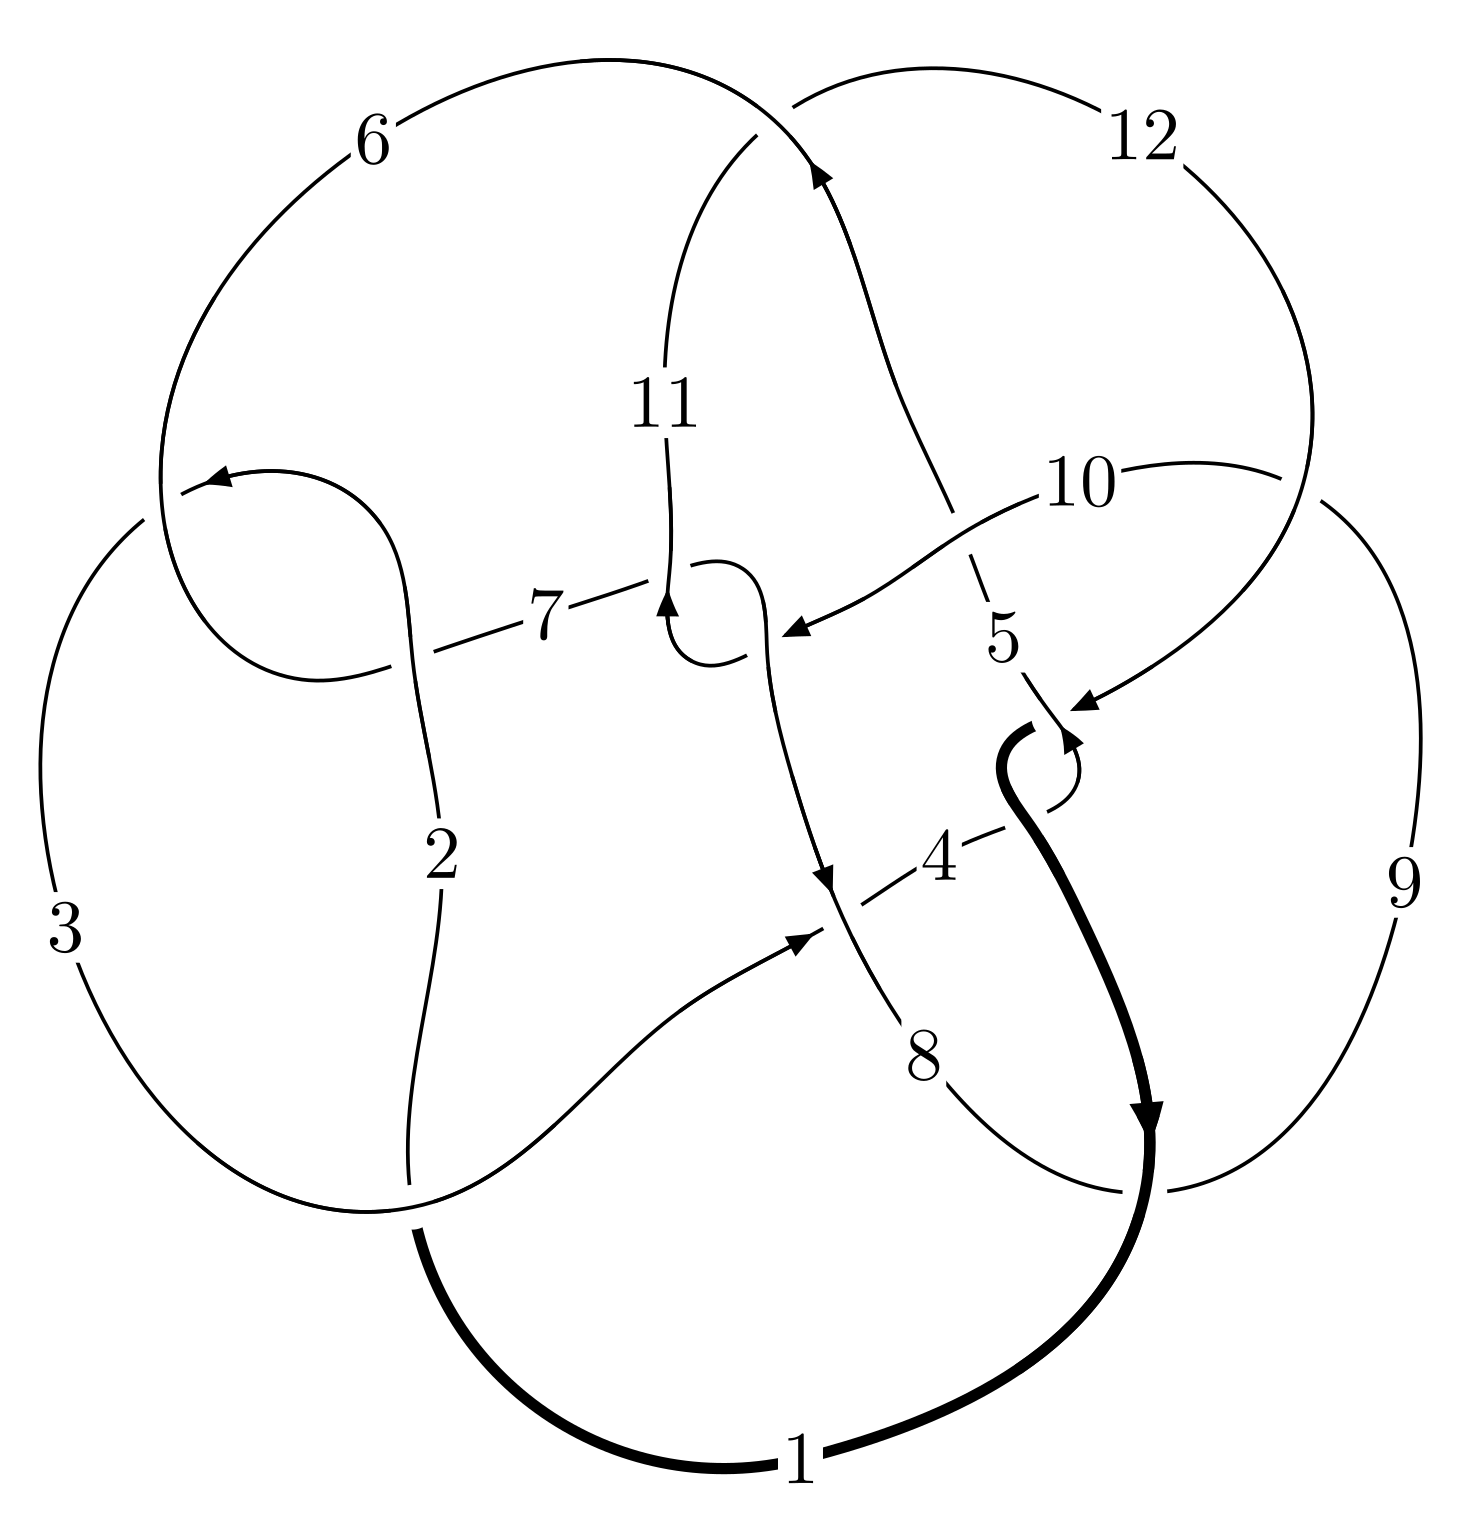
\includegraphics[width=112pt]{../../../GIT/diagram.site/Diagrams/png/2523_12n_0434.png}\\
\ \ \ A knot diagram\footnotemark}&
\allowdisplaybreaks
\textbf{Linearized knot diagam} \\
\cline{2-2}
 &
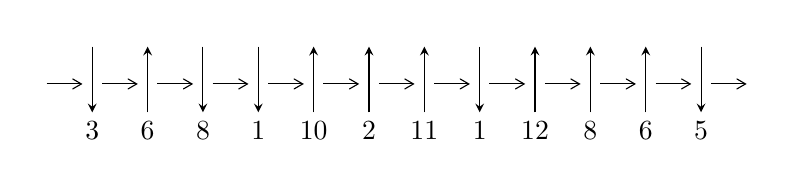
\begin{tikzpicture}[x=20pt, y=17pt]
	% nodes
	\node (C0) at (0, 0) {};
	\node (C1) at (1, 0) {};
	\node (C1U) at (1, +1) {};
	\node (C1D) at (1, -1) {3};

	\node (C2) at (2, 0) {};
	\node (C2U) at (2, +1) {};
	\node (C2D) at (2, -1) {6};

	\node (C3) at (3, 0) {};
	\node (C3U) at (3, +1) {};
	\node (C3D) at (3, -1) {8};

	\node (C4) at (4, 0) {};
	\node (C4U) at (4, +1) {};
	\node (C4D) at (4, -1) {1};

	\node (C5) at (5, 0) {};
	\node (C5U) at (5, +1) {};
	\node (C5D) at (5, -1) {10};

	\node (C6) at (6, 0) {};
	\node (C6U) at (6, +1) {};
	\node (C6D) at (6, -1) {2};

	\node (C7) at (7, 0) {};
	\node (C7U) at (7, +1) {};
	\node (C7D) at (7, -1) {11};

	\node (C8) at (8, 0) {};
	\node (C8U) at (8, +1) {};
	\node (C8D) at (8, -1) {1};

	\node (C9) at (9, 0) {};
	\node (C9U) at (9, +1) {};
	\node (C9D) at (9, -1) {12};

	\node (C10) at (10, 0) {};
	\node (C10U) at (10, +1) {};
	\node (C10D) at (10, -1) {8};

	\node (C11) at (11, 0) {};
	\node (C11U) at (11, +1) {};
	\node (C11D) at (11, -1) {6};

	\node (C12) at (12, 0) {};
	\node (C12U) at (12, +1) {};
	\node (C12D) at (12, -1) {5};
	\node (C13) at (13, 0) {};

	% arrows
	\draw[->,>={angle 60}]
	(C0) edge (C1) (C1) edge (C2) (C2) edge (C3) (C3) edge (C4) (C4) edge (C5) (C5) edge (C6) (C6) edge (C7) (C7) edge (C8) (C8) edge (C9) (C9) edge (C10) (C10) edge (C11) (C11) edge (C12) (C12) edge (C13) ;	\draw[->,>=stealth]
	(C1U) edge (C1D) (C2D) edge (C2U) (C3U) edge (C3D) (C4U) edge (C4D) (C5D) edge (C5U) (C6D) edge (C6U) (C7D) edge (C7U) (C8U) edge (C8D) (C9D) edge (C9U) (C10D) edge (C10U) (C11D) edge (C11U) (C12U) edge (C12D) ;
	\end{tikzpicture} \\
\hhline{~~} \\& 
\textbf{Solving Sequence} \\ \cline{2-2} 
 &
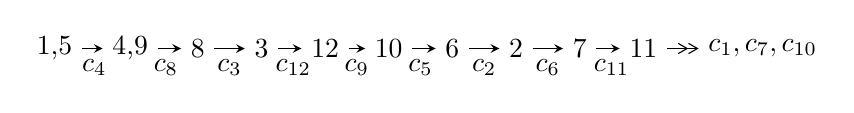
\begin{tikzpicture}[x=23pt, y=7pt]
	% node
	\node (A0) at (-1/8, 0) {1,5};
	\node (A1) at (17/16, 0) {4,9};
	\node (A2) at (17/8, 0) {8};
	\node (A3) at (25/8, 0) {3};
	\node (A4) at (33/8, 0) {12};
	\node (A5) at (41/8, 0) {10};
	\node (A6) at (49/8, 0) {6};
	\node (A7) at (57/8, 0) {2};
	\node (A8) at (65/8, 0) {7};
	\node (A9) at (73/8, 0) {11};
	\node (C1) at (1/2, -1) {$c_{4}$};
	\node (C2) at (13/8, -1) {$c_{8}$};
	\node (C3) at (21/8, -1) {$c_{3}$};
	\node (C4) at (29/8, -1) {$c_{12}$};
	\node (C5) at (37/8, -1) {$c_{9}$};
	\node (C6) at (45/8, -1) {$c_{5}$};
	\node (C7) at (53/8, -1) {$c_{2}$};
	\node (C8) at (61/8, -1) {$c_{6}$};
	\node (C9) at (69/8, -1) {$c_{11}$};
	\node (A10) at (11, 0) {$c_{1},c_{7},c_{10}$};

	% edge
	\draw[->,>=stealth]	
	(A0) edge (A1) (A1) edge (A2) (A2) edge (A3) (A3) edge (A4) (A4) edge (A5) (A5) edge (A6) (A6) edge (A7) (A7) edge (A8) (A8) edge (A9) ;
	\draw[->>,>={angle 60}]	
	(A9) edge (A10);
\end{tikzpicture} \\ 

\end{tabular} \\

\footnotetext{
The image of knot diagram is generated by the software ``\textbf{Draw programme}" developed by Andrew Bartholomew(\url{http://www.layer8.co.uk/maths/draw/index.htm\#Running-draw}), where we modified some parts for our purpose(\url{https://github.com/CATsTAILs/LinksPainter}).
}\phantom \\ \newline 
\centering \textbf{Ideals for irreducible components\footnotemark of $X_{\text{par}}$} 
 
\begin{align*}
I^u_{1}&=\langle 
1.15244\times10^{89} u^{53}-2.36305\times10^{89} u^{52}+\cdots+1.14353\times10^{89} b+6.98962\times10^{89},\\
\phantom{I^u_{1}}&\phantom{= \langle  }-2.35956\times10^{90} u^{53}+4.56370\times10^{90} u^{52}+\cdots+8.00468\times10^{89} a-4.87445\times10^{90},\;u^{54}-3 u^{53}+\cdots-3 u+1\rangle \\
I^u_{2}&=\langle 
13421 u^{13}+20820 u^{12}+\cdots+17217 b-11948,\;655 u^{13}+3102 u^{12}+\cdots+5739 a+3767,\\
\phantom{I^u_{2}}&\phantom{= \langle  }u^{14}+2 u^{13}+4 u^{12}+3 u^{11}+6 u^{10}+6 u^9+14 u^8+14 u^7+19 u^6+14 u^5+10 u^4+2 u^3+3 u^2+1\rangle \\
I^u_{3}&=\langle 
u^3+2 b-3,\;u^3+2 a-3,\;u^4+u^3+2 u^2- u+1\rangle \\
I^u_{4}&=\langle 
u^2+b+1,\;u^2+a+1,\;u^4+u^3+2 u^2+2 u+1\rangle \\
\\
\end{align*}
\raggedright * 4 irreducible components of $\dim_{\mathbb{C}}=0$, with total 76 representations.\\
\footnotetext{All coefficients of polynomials are rational numbers. But the coefficients are sometimes approximated in decimal forms when there is not enough margin.}
\newpage
\renewcommand{\arraystretch}{1}
\centering \section*{I. $I^u_{1}= \langle 1.15\times10^{89} u^{53}-2.36\times10^{89} u^{52}+\cdots+1.14\times10^{89} b+6.99\times10^{89},\;-2.36\times10^{90} u^{53}+4.56\times10^{90} u^{52}+\cdots+8.00\times10^{89} a-4.87\times10^{90},\;u^{54}-3 u^{53}+\cdots-3 u+1 \rangle$}
\flushleft \textbf{(i) Arc colorings}\\
\begin{tabular}{m{7pt} m{180pt} m{7pt} m{180pt} }
\flushright $a_{1}=$&$\begin{pmatrix}0\\u\end{pmatrix}$ \\
\flushright $a_{5}=$&$\begin{pmatrix}1\\0\end{pmatrix}$ \\
\flushright $a_{4}=$&$\begin{pmatrix}1\\- u^2\end{pmatrix}$ \\
\flushright $a_{9}=$&$\begin{pmatrix}2.94773 u^{53}-5.70129 u^{52}+\cdots-14.5124 u+6.08949\\-1.00780 u^{53}+2.06646 u^{52}+\cdots+15.3054 u-6.11234\end{pmatrix}$ \\
\flushright $a_{8}=$&$\begin{pmatrix}2.94773 u^{53}-5.70129 u^{52}+\cdots-14.5124 u+6.08949\\-0.287284 u^{53}+0.699825 u^{52}+\cdots+8.82747 u-2.97046\end{pmatrix}$ \\
\flushright $a_{3}=$&$\begin{pmatrix}-1.97603 u^{53}+4.47321 u^{52}+\cdots+27.0023 u-13.6868\\0.915616 u^{53}-1.04433 u^{52}+\cdots-14.8536 u+3.07727\end{pmatrix}$ \\
\flushright $a_{12}=$&$\begin{pmatrix}u\\u\end{pmatrix}$ \\
\flushright $a_{10}=$&$\begin{pmatrix}4.21790 u^{53}-8.54770 u^{52}+\cdots-22.8533 u+10.1883\\0.262380 u^{53}-0.779944 u^{52}+\cdots+6.96448 u-2.01353\end{pmatrix}$ \\
\flushright $a_{6}=$&$\begin{pmatrix}5.26626 u^{53}-18.3261 u^{52}+\cdots+62.9922 u-13.9709\\0.751703 u^{53}-1.91257 u^{52}+\cdots+2.33641 u-1.75467\end{pmatrix}$ \\
\flushright $a_{2}=$&$\begin{pmatrix}-11.3826 u^{53}+30.2001 u^{52}+\cdots+7.41660 u-26.3662\\0.520213 u^{53}-0.0746840 u^{52}+\cdots-27.1247 u+3.86789\end{pmatrix}$ \\
\flushright $a_{7}=$&$\begin{pmatrix}-8.72344 u^{53}+33.9754 u^{52}+\cdots-130.452 u+31.2985\\3.58969 u^{53}-10.8714 u^{52}+\cdots+6.78177 u+2.52277\end{pmatrix}$ \\
\flushright $a_{11}=$&$\begin{pmatrix}12.7906 u^{53}-37.1295 u^{52}+\cdots+18.7277 u+3.70834\\1.17501 u^{53}-4.52802 u^{52}+\cdots+14.7445 u-5.03833\end{pmatrix}$\\&\end{tabular}
\flushleft \textbf{(ii) Obstruction class $= -1$}\\~\\
\flushleft \textbf{(iii) Cusp Shapes $= 1.14333 u^{53}-0.924812 u^{52}+\cdots-6.63399 u+6.45142$}\\~\\
\newpage\renewcommand{\arraystretch}{1}
\flushleft \textbf{(iv) u-Polynomials at the component}\newline \\
\begin{tabular}{m{50pt}|m{274pt}}
Crossings & \hspace{64pt}u-Polynomials at each crossing \\
\hline $$\begin{aligned}c_{1}\end{aligned}$$&$\begin{aligned}
&u^{54}+43 u^{53}+\cdots+3692 u+441
\end{aligned}$\\
\hline $$\begin{aligned}c_{2},c_{6}\end{aligned}$$&$\begin{aligned}
&u^{54}- u^{53}+\cdots-26 u+21
\end{aligned}$\\
\hline $$\begin{aligned}c_{3}\end{aligned}$$&$\begin{aligned}
&u^{54}-25 u^{52}+\cdots+2432 u+1856
\end{aligned}$\\
\hline $$\begin{aligned}c_{4},c_{12}\end{aligned}$$&$\begin{aligned}
&u^{54}-3 u^{53}+\cdots-3 u+1
\end{aligned}$\\
\hline $$\begin{aligned}c_{5}\end{aligned}$$&$\begin{aligned}
&u^{54}+2 u^{53}+\cdots+153 u+47
\end{aligned}$\\
\hline $$\begin{aligned}c_{7},c_{10}\end{aligned}$$&$\begin{aligned}
&u^{54}+u^{53}+\cdots-2486 u+121
\end{aligned}$\\
\hline $$\begin{aligned}c_{8}\end{aligned}$$&$\begin{aligned}
&u^{54}+5 u^{53}+\cdots-17089 u+1801
\end{aligned}$\\
\hline $$\begin{aligned}c_{9}\end{aligned}$$&$\begin{aligned}
&u^{54}+9 u^{53}+\cdots+3712 u+768
\end{aligned}$\\
\hline $$\begin{aligned}c_{11}\end{aligned}$$&$\begin{aligned}
&u^{54}+u^{53}+\cdots+1004850 u+134807
\end{aligned}$\\
\hline
\end{tabular}\\~\\
\newpage\renewcommand{\arraystretch}{1}
\flushleft \textbf{(v) Riley Polynomials at the component}\newline \\
\begin{tabular}{m{50pt}|m{274pt}}
Crossings & \hspace{64pt}Riley Polynomials at each crossing \\
\hline $$\begin{aligned}c_{1}\end{aligned}$$&$\begin{aligned}
&y^{54}-49 y^{53}+\cdots+4263152 y+194481
\end{aligned}$\\
\hline $$\begin{aligned}c_{2},c_{6}\end{aligned}$$&$\begin{aligned}
&y^{54}+43 y^{53}+\cdots+3692 y+441
\end{aligned}$\\
\hline $$\begin{aligned}c_{3}\end{aligned}$$&$\begin{aligned}
&y^{54}-50 y^{53}+\cdots-42856448 y+3444736
\end{aligned}$\\
\hline $$\begin{aligned}c_{4},c_{12}\end{aligned}$$&$\begin{aligned}
&y^{54}+11 y^{53}+\cdots+41 y+1
\end{aligned}$\\
\hline $$\begin{aligned}c_{5}\end{aligned}$$&$\begin{aligned}
&y^{54}-6 y^{53}+\cdots+27633 y+2209
\end{aligned}$\\
\hline $$\begin{aligned}c_{7},c_{10}\end{aligned}$$&$\begin{aligned}
&y^{54}+65 y^{53}+\cdots-587818 y+14641
\end{aligned}$\\
\hline $$\begin{aligned}c_{8}\end{aligned}$$&$\begin{aligned}
&y^{54}-63 y^{53}+\cdots+140310537 y+3243601
\end{aligned}$\\
\hline $$\begin{aligned}c_{9}\end{aligned}$$&$\begin{aligned}
&y^{54}+31 y^{53}+\cdots-9355264 y+589824
\end{aligned}$\\
\hline $$\begin{aligned}c_{11}\end{aligned}$$&$\begin{aligned}
&y^{54}+75 y^{53}+\cdots-92128132162 y+18172927249
\end{aligned}$\\
\hline
\end{tabular}\\~\\
\newpage\flushleft \textbf{(vi) Complex Volumes and Cusp Shapes}
$$\begin{array}{c|c|c}  
\text{Solutions to }I^u_{1}& \I (\text{vol} + \sqrt{-1}CS) & \text{Cusp shape}\\
 \hline 
\begin{aligned}
u &= -0.037373 + 1.006010 I \\
a &= \phantom{-}1.030200 + 0.062419 I \\
b &= -0.490474 - 0.580472 I\end{aligned}
 & \phantom{-}2.85970 + 0.80963 I & \phantom{-}6.77195 + 0.29503 I \\ \hline\begin{aligned}
u &= -0.037373 - 1.006010 I \\
a &= \phantom{-}1.030200 - 0.062419 I \\
b &= -0.490474 + 0.580472 I\end{aligned}
 & \phantom{-}2.85970 - 0.80963 I & \phantom{-}6.77195 - 0.29503 I \\ \hline\begin{aligned}
u &= -0.543124 + 0.777830 I \\
a &= -0.471157 + 0.381929 I \\
b &= -0.50611 + 1.96562 I\end{aligned}
 & -7.74259 + 6.23460 I & -0.70370 - 6.97900 I \\ \hline\begin{aligned}
u &= -0.543124 - 0.777830 I \\
a &= -0.471157 - 0.381929 I \\
b &= -0.50611 - 1.96562 I\end{aligned}
 & -7.74259 - 6.23460 I & -0.70370 + 6.97900 I \\ \hline\begin{aligned}
u &= -0.431004 + 0.822553 I \\
a &= -1.029580 + 0.012079 I \\
b &= -0.807592 + 0.331900 I\end{aligned}
 & -0.65107 + 2.00888 I & \phantom{-}0.23679 - 4.07426 I \\ \hline\begin{aligned}
u &= -0.431004 - 0.822553 I \\
a &= -1.029580 - 0.012079 I \\
b &= -0.807592 - 0.331900 I\end{aligned}
 & -0.65107 - 2.00888 I & \phantom{-}0.23679 + 4.07426 I \\ \hline\begin{aligned}
u &= -0.795980 + 0.436234 I \\
a &= -0.277873 + 0.419648 I \\
b &= -0.318797 - 0.205145 I\end{aligned}
 & -1.27040 + 1.87667 I & -3.97787 - 4.44520 I \\ \hline\begin{aligned}
u &= -0.795980 - 0.436234 I \\
a &= -0.277873 - 0.419648 I \\
b &= -0.318797 + 0.205145 I\end{aligned}
 & -1.27040 - 1.87667 I & -3.97787 + 4.44520 I \\ \hline\begin{aligned}
u &= \phantom{-}0.527527 + 1.001810 I \\
a &= \phantom{-}1.149730 - 0.365464 I \\
b &= \phantom{-}1.53010 - 0.50566 I\end{aligned}
 & -2.71697 - 1.97809 I & \phantom{-0.000000 -}0. + 2.58049 I \\ \hline\begin{aligned}
u &= \phantom{-}0.527527 - 1.001810 I \\
a &= \phantom{-}1.149730 + 0.365464 I \\
b &= \phantom{-}1.53010 + 0.50566 I\end{aligned}
 & -2.71697 + 1.97809 I & \phantom{-0.000000 } 0. - 2.58049 I\\
 \hline 
 \end{array}$$\newpage$$\begin{array}{c|c|c}  
\text{Solutions to }I^u_{1}& \I (\text{vol} + \sqrt{-1}CS) & \text{Cusp shape}\\
 \hline 
\begin{aligned}
u &= -0.918205 + 0.762698 I \\
a &= -1.118580 - 0.397034 I \\
b &= -1.122090 + 0.488407 I\end{aligned}
 & -2.04155 + 2.12181 I & \phantom{-0.000000 } 0 \\ \hline\begin{aligned}
u &= -0.918205 - 0.762698 I \\
a &= -1.118580 + 0.397034 I \\
b &= -1.122090 - 0.488407 I\end{aligned}
 & -2.04155 - 2.12181 I & \phantom{-0.000000 } 0 \\ \hline\begin{aligned}
u &= -0.364190 + 1.145600 I \\
a &= -0.442213 + 0.376301 I \\
b &= \phantom{-}0.400143 - 0.343043 I\end{aligned}
 & \phantom{-}3.58333 + 4.89977 I & \phantom{-0.000000 } 0. - 7.27006 I \\ \hline\begin{aligned}
u &= -0.364190 - 1.145600 I \\
a &= -0.442213 - 0.376301 I \\
b &= \phantom{-}0.400143 + 0.343043 I\end{aligned}
 & \phantom{-}3.58333 - 4.89977 I & \phantom{-0.000000 -}0. + 7.27006 I \\ \hline\begin{aligned}
u &= \phantom{-}0.960632 + 0.774462 I \\
a &= \phantom{-}1.13070 - 0.89501 I \\
b &= \phantom{-}1.59243 + 0.09416 I\end{aligned}
 & -7.46820 + 0.80208 I & \phantom{-0.000000 } 0 \\ \hline\begin{aligned}
u &= \phantom{-}0.960632 - 0.774462 I \\
a &= \phantom{-}1.13070 + 0.89501 I \\
b &= \phantom{-}1.59243 - 0.09416 I\end{aligned}
 & -7.46820 - 0.80208 I & \phantom{-0.000000 } 0 \\ \hline\begin{aligned}
u &= \phantom{-}0.600991 + 0.467590 I \\
a &= \phantom{-}0.158333 - 0.973691 I \\
b &= \phantom{-}0.100996 + 0.808006 I\end{aligned}
 & -3.72491 - 3.82211 I & \phantom{-}6.70276 + 1.18963 I \\ \hline\begin{aligned}
u &= \phantom{-}0.600991 - 0.467590 I \\
a &= \phantom{-}0.158333 + 0.973691 I \\
b &= \phantom{-}0.100996 - 0.808006 I\end{aligned}
 & -3.72491 + 3.82211 I & \phantom{-}6.70276 - 1.18963 I \\ \hline\begin{aligned}
u &= \phantom{-}0.979992 + 0.797814 I \\
a &= -1.43891 + 0.26324 I \\
b &= -1.97461 - 0.43491 I\end{aligned}
 & -15.3307 - 5.7207 I & \phantom{-0.000000 } 0 \\ \hline\begin{aligned}
u &= \phantom{-}0.979992 - 0.797814 I \\
a &= -1.43891 - 0.26324 I \\
b &= -1.97461 + 0.43491 I\end{aligned}
 & -15.3307 + 5.7207 I & \phantom{-0.000000 } 0\\
 \hline 
 \end{array}$$\newpage$$\begin{array}{c|c|c}  
\text{Solutions to }I^u_{1}& \I (\text{vol} + \sqrt{-1}CS) & \text{Cusp shape}\\
 \hline 
\begin{aligned}
u &= \phantom{-}0.187854 + 1.250900 I \\
a &= -0.186276 + 0.095635 I \\
b &= -0.859056 + 0.377021 I\end{aligned}
 & -0.658796 + 0.749765 I & \phantom{-0.000000 } 0 \\ \hline\begin{aligned}
u &= \phantom{-}0.187854 - 1.250900 I \\
a &= -0.186276 - 0.095635 I \\
b &= -0.859056 - 0.377021 I\end{aligned}
 & -0.658796 - 0.749765 I & \phantom{-0.000000 } 0 \\ \hline\begin{aligned}
u &= -0.247033 + 0.676299 I \\
a &= -0.301606 + 0.279111 I \\
b &= -0.365687 + 0.725077 I\end{aligned}
 & -0.05790 + 1.76249 I & \phantom{-}0.05580 - 5.36659 I \\ \hline\begin{aligned}
u &= -0.247033 - 0.676299 I \\
a &= -0.301606 - 0.279111 I \\
b &= -0.365687 - 0.725077 I\end{aligned}
 & -0.05790 - 1.76249 I & \phantom{-}0.05580 + 5.36659 I \\ \hline\begin{aligned}
u &= \phantom{-}1.098870 + 0.656535 I \\
a &= \phantom{-}1.55286 - 0.44234 I \\
b &= \phantom{-}1.158690 + 0.463793 I\end{aligned}
 & -4.13666 - 6.24317 I & \phantom{-0.000000 } 0 \\ \hline\begin{aligned}
u &= \phantom{-}1.098870 - 0.656535 I \\
a &= \phantom{-}1.55286 + 0.44234 I \\
b &= \phantom{-}1.158690 - 0.463793 I\end{aligned}
 & -4.13666 + 6.24317 I & \phantom{-0.000000 } 0 \\ \hline\begin{aligned}
u &= -0.697329 + 0.022686 I \\
a &= -1.38730 + 3.11746 I \\
b &= \phantom{-}0.181432 + 0.532548 I\end{aligned}
 & -9.05440 - 2.92567 I & -6.42699 + 0.09398 I \\ \hline\begin{aligned}
u &= -0.697329 - 0.022686 I \\
a &= -1.38730 - 3.11746 I \\
b &= \phantom{-}0.181432 - 0.532548 I\end{aligned}
 & -9.05440 + 2.92567 I & -6.42699 - 0.09398 I \\ \hline\begin{aligned}
u &= \phantom{-}1.026470 + 0.845684 I \\
a &= -1.40395 + 1.00681 I \\
b &= -1.220970 - 0.303738 I\end{aligned}
 & -4.13120 - 4.24024 I & \phantom{-0.000000 } 0 \\ \hline\begin{aligned}
u &= \phantom{-}1.026470 - 0.845684 I \\
a &= -1.40395 - 1.00681 I \\
b &= -1.220970 + 0.303738 I\end{aligned}
 & -4.13120 + 4.24024 I & \phantom{-0.000000 } 0\\
 \hline 
 \end{array}$$\newpage$$\begin{array}{c|c|c}  
\text{Solutions to }I^u_{1}& \I (\text{vol} + \sqrt{-1}CS) & \text{Cusp shape}\\
 \hline 
\begin{aligned}
u &= \phantom{-}0.837598 + 1.066200 I \\
a &= -1.124140 + 0.742986 I \\
b &= -1.77532 - 0.42316 I\end{aligned}
 & -6.55172 - 7.42273 I & \phantom{-0.000000 } 0 \\ \hline\begin{aligned}
u &= \phantom{-}0.837598 - 1.066200 I \\
a &= -1.124140 - 0.742986 I \\
b &= -1.77532 + 0.42316 I\end{aligned}
 & -6.55172 + 7.42273 I & \phantom{-0.000000 } 0 \\ \hline\begin{aligned}
u &= \phantom{-}0.815947 + 1.102350 I \\
a &= \phantom{-}0.53489 - 1.31244 I \\
b &= \phantom{-}1.53981 - 0.09220 I\end{aligned}
 & -14.3214 - 0.9597 I & \phantom{-0.000000 } 0 \\ \hline\begin{aligned}
u &= \phantom{-}0.815947 - 1.102350 I \\
a &= \phantom{-}0.53489 + 1.31244 I \\
b &= \phantom{-}1.53981 + 0.09220 I\end{aligned}
 & -14.3214 + 0.9597 I & \phantom{-0.000000 } 0 \\ \hline\begin{aligned}
u &= -1.131240 + 0.821749 I \\
a &= \phantom{-}1.105120 + 0.458003 I \\
b &= \phantom{-}1.61964 - 0.06450 I\end{aligned}
 & -10.58060 - 0.64727 I & \phantom{-0.000000 } 0 \\ \hline\begin{aligned}
u &= -1.131240 - 0.821749 I \\
a &= \phantom{-}1.105120 - 0.458003 I \\
b &= \phantom{-}1.61964 + 0.06450 I\end{aligned}
 & -10.58060 + 0.64727 I & \phantom{-0.000000 } 0 \\ \hline\begin{aligned}
u &= -0.090452 + 0.526330 I \\
a &= \phantom{-}1.120460 + 0.305656 I \\
b &= \phantom{-}0.74665 - 1.44801 I\end{aligned}
 & \phantom{-}1.157250 - 0.155163 I & \phantom{-}7.37161 - 1.36723 I \\ \hline\begin{aligned}
u &= -0.090452 - 0.526330 I \\
a &= \phantom{-}1.120460 - 0.305656 I \\
b &= \phantom{-}0.74665 + 1.44801 I\end{aligned}
 & \phantom{-}1.157250 + 0.155163 I & \phantom{-}7.37161 + 1.36723 I \\ \hline\begin{aligned}
u &= -0.93222 + 1.15582 I \\
a &= -0.936289 - 0.829653 I \\
b &= -1.54017 + 0.35175 I\end{aligned}
 & -9.48565 + 8.12595 I & \phantom{-0.000000 } 0 \\ \hline\begin{aligned}
u &= -0.93222 - 1.15582 I \\
a &= -0.936289 + 0.829653 I \\
b &= -1.54017 - 0.35175 I\end{aligned}
 & -9.48565 - 8.12595 I & \phantom{-0.000000 } 0\\
 \hline 
 \end{array}$$\newpage$$\begin{array}{c|c|c}  
\text{Solutions to }I^u_{1}& \I (\text{vol} + \sqrt{-1}CS) & \text{Cusp shape}\\
 \hline 
\begin{aligned}
u &= -0.94640 + 1.15434 I \\
a &= \phantom{-}0.757645 + 0.359126 I \\
b &= \phantom{-}0.951028 - 0.386906 I\end{aligned}
 & -0.63092 + 4.66377 I & \phantom{-0.000000 } 0 \\ \hline\begin{aligned}
u &= -0.94640 - 1.15434 I \\
a &= \phantom{-}0.757645 - 0.359126 I \\
b &= \phantom{-}0.951028 + 0.386906 I\end{aligned}
 & -0.63092 - 4.66377 I & \phantom{-0.000000 } 0 \\ \hline\begin{aligned}
u &= -0.055729 + 0.503312 I \\
a &= -1.96871 - 3.65912 I \\
b &= \phantom{-}0.886771 + 0.795520 I\end{aligned}
 & -8.54356 - 3.22703 I & \phantom{-}3.94778 - 2.72438 I \\ \hline\begin{aligned}
u &= -0.055729 - 0.503312 I \\
a &= -1.96871 + 3.65912 I \\
b &= \phantom{-}0.886771 - 0.795520 I\end{aligned}
 & -8.54356 + 3.22703 I & \phantom{-}3.94778 + 2.72438 I \\ \hline\begin{aligned}
u &= \phantom{-}0.99851 + 1.13262 I \\
a &= \phantom{-}1.34755 - 0.60244 I \\
b &= \phantom{-}1.70196 + 0.68361 I\end{aligned}
 & -14.2209 - 14.9873 I & \phantom{-0.000000 } 0 \\ \hline\begin{aligned}
u &= \phantom{-}0.99851 - 1.13262 I \\
a &= \phantom{-}1.34755 + 0.60244 I \\
b &= \phantom{-}1.70196 - 0.68361 I\end{aligned}
 & -14.2209 + 14.9873 I & \phantom{-0.000000 } 0 \\ \hline\begin{aligned}
u &= \phantom{-}1.19097 + 0.94277 I \\
a &= -0.950142 + 0.775950 I \\
b &= -1.54086 + 0.39585 I\end{aligned}
 & -14.9446 + 7.1061 I & \phantom{-0.000000 } 0 \\ \hline\begin{aligned}
u &= \phantom{-}1.19097 - 0.94277 I \\
a &= -0.950142 - 0.775950 I \\
b &= -1.54086 - 0.39585 I\end{aligned}
 & -14.9446 - 7.1061 I & \phantom{-0.000000 } 0 \\ \hline\begin{aligned}
u &= -0.79135 + 1.35810 I \\
a &= \phantom{-}0.524839 + 0.318013 I \\
b &= \phantom{-}0.921922 - 0.092922 I\end{aligned}
 & -0.47705 + 4.55318 I & \phantom{-0.000000 } 0 \\ \hline\begin{aligned}
u &= -0.79135 - 1.35810 I \\
a &= \phantom{-}0.524839 - 0.318013 I \\
b &= \phantom{-}0.921922 + 0.092922 I\end{aligned}
 & -0.47705 - 4.55318 I & \phantom{-0.000000 } 0\\
 \hline 
 \end{array}$$\newpage$$\begin{array}{c|c|c}  
\text{Solutions to }I^u_{1}& \I (\text{vol} + \sqrt{-1}CS) & \text{Cusp shape}\\
 \hline 
\begin{aligned}
u &= \phantom{-}0.124133 + 0.402569 I \\
a &= \phantom{-}0.92386 + 1.37352 I \\
b &= \phantom{-}0.575765 - 0.613700 I\end{aligned}
 & \phantom{-}1.34934 - 0.45303 I & \phantom{-}8.18333 + 1.54346 I \\ \hline\begin{aligned}
u &= \phantom{-}0.124133 - 0.402569 I \\
a &= \phantom{-}0.92386 - 1.37352 I \\
b &= \phantom{-}0.575765 + 0.613700 I\end{aligned}
 & \phantom{-}1.34934 + 0.45303 I & \phantom{-}8.18333 - 1.54346 I \\ \hline\begin{aligned}
u &= \phantom{-}0.132130 + 0.214010 I \\
a &= -4.29946 + 0.59400 I \\
b &= -1.385600 - 0.232769 I\end{aligned}
 & -0.15771 - 3.49876 I & \phantom{-}0.819601 - 0.411516 I \\ \hline\begin{aligned}
u &= \phantom{-}0.132130 - 0.214010 I \\
a &= -4.29946 - 0.59400 I \\
b &= -1.385600 + 0.232769 I\end{aligned}
 & -0.15771 + 3.49876 I & \phantom{-}0.819601 + 0.411516 I\\
 \hline 
 \end{array}$$\newpage\newpage\renewcommand{\arraystretch}{1}
\centering \section*{II. $I^u_{2}= \langle 13421 u^{13}+20820 u^{12}+\cdots+17217 b-11948,\;655 u^{13}+3102 u^{12}+\cdots+5739 a+3767,\;u^{14}+2 u^{13}+\cdots+3 u^2+1 \rangle$}
\flushleft \textbf{(i) Arc colorings}\\
\begin{tabular}{m{7pt} m{180pt} m{7pt} m{180pt} }
\flushright $a_{1}=$&$\begin{pmatrix}0\\u\end{pmatrix}$ \\
\flushright $a_{5}=$&$\begin{pmatrix}1\\0\end{pmatrix}$ \\
\flushright $a_{4}=$&$\begin{pmatrix}1\\- u^2\end{pmatrix}$ \\
\flushright $a_{9}=$&$\begin{pmatrix}-0.114131 u^{13}-0.540512 u^{12}+\cdots-4.39449 u-0.656386\\-0.779520 u^{13}-1.20927 u^{12}+\cdots-0.757507 u+0.693965\end{pmatrix}$ \\
\flushright $a_{8}=$&$\begin{pmatrix}-0.114131 u^{13}-0.540512 u^{12}+\cdots-4.39449 u-0.656386\\-0.369518 u^{13}-0.334727 u^{12}+\cdots-0.871638 u+0.381716\end{pmatrix}$ \\
\flushright $a_{3}=$&$\begin{pmatrix}1.42975 u^{13}+3.35738 u^{12}+\cdots+4.06354 u+0.526514\\0.404310 u^{13}+1.03537 u^{12}+\cdots+0.381716 u+1.36952\end{pmatrix}$ \\
\flushright $a_{12}=$&$\begin{pmatrix}u\\u\end{pmatrix}$ \\
\flushright $a_{10}=$&$\begin{pmatrix}0.448220 u^{13}+0.508974 u^{12}+\cdots-3.72910 u-1.31841\\-0.217169 u^{13}-0.159784 u^{12}+\cdots-0.0921183 u+0.0319452\end{pmatrix}$ \\
\flushright $a_{6}=$&$\begin{pmatrix}1.04374 u^{13}+2.01934 u^{12}+\cdots-1.69768 u-1.46297\\0.349771 u^{13}+0.851891 u^{12}+\cdots+0.693965 u+0.779520\end{pmatrix}$ \\
\flushright $a_{2}=$&$\begin{pmatrix}2.37672 u^{13}+6.11082 u^{12}+\cdots+6.79526 u+0.653598\\-0.0935703 u^{13}+0.0622060 u^{12}+\cdots-0.144799 u+1.79927\end{pmatrix}$ \\
\flushright $a_{7}=$&$\begin{pmatrix}-1.98949 u^{13}-3.59296 u^{12}+\cdots+6.07400 u+5.76122\\-0.589998 u^{13}-1.12546 u^{12}+\cdots-4.11413 u-0.312250\end{pmatrix}$ \\
\flushright $a_{11}=$&$\begin{pmatrix}-1.79427 u^{13}-4.66998 u^{12}+\cdots-2.77847 u+1.07324\\0.562351 u^{13}+1.04949 u^{12}+\cdots+0.665389 u-0.662020\end{pmatrix}$\\&\end{tabular}
\flushleft \textbf{(ii) Obstruction class $= 1$}\\~\\
\flushleft \textbf{(iii) Cusp Shapes $= -\frac{2746}{5739} u^{13}+\frac{4976}{1913} u^{12}+\cdots+\frac{19957}{5739} u+\frac{38557}{5739}$}\\~\\
\newpage\renewcommand{\arraystretch}{1}
\flushleft \textbf{(iv) u-Polynomials at the component}\newline \\
\begin{tabular}{m{50pt}|m{274pt}}
Crossings & \hspace{64pt}u-Polynomials at each crossing \\
\hline $$\begin{aligned}c_{1}\end{aligned}$$&$\begin{aligned}
&u^{14}-10 u^{13}+\cdots-16 u+1
\end{aligned}$\\
\hline $$\begin{aligned}c_{2}\end{aligned}$$&$\begin{aligned}
&u^{14}-4 u^{13}+\cdots-2 u+1
\end{aligned}$\\
\hline $$\begin{aligned}c_{3}\end{aligned}$$&$\begin{aligned}
&u^{14}- u^{12}+u^{11}- u^{10}+5 u^8-3 u^7-5 u^6+3 u^5+4 u^4- u^3-3 u^2+1
\end{aligned}$\\
\hline $$\begin{aligned}c_{4}\end{aligned}$$&$\begin{aligned}
&u^{14}+2 u^{13}+\cdots+3 u^2+1
\end{aligned}$\\
\hline $$\begin{aligned}c_{5}\end{aligned}$$&$\begin{aligned}
&u^{14}-3 u^{12}+u^{11}+4 u^{10}-3 u^9-5 u^8+3 u^7+5 u^6- u^4- u^3- u^2+1
\end{aligned}$\\
\hline $$\begin{aligned}c_{6}\end{aligned}$$&$\begin{aligned}
&u^{14}+4 u^{13}+\cdots+2 u+1
\end{aligned}$\\
\hline $$\begin{aligned}c_{7}\end{aligned}$$&$\begin{aligned}
&u^{14}+6 u^{12}+\cdots-2 u+1
\end{aligned}$\\
\hline $$\begin{aligned}c_{8}\end{aligned}$$&$\begin{aligned}
&u^{14}+4 u^{13}+\cdots+55 u+19
\end{aligned}$\\
\hline $$\begin{aligned}c_{9}\end{aligned}$$&$\begin{aligned}
&u^{14}+2 u^{13}+\cdots+1130 u+325
\end{aligned}$\\
\hline $$\begin{aligned}c_{10}\end{aligned}$$&$\begin{aligned}
&u^{14}+6 u^{12}+\cdots+2 u+1
\end{aligned}$\\
\hline $$\begin{aligned}c_{11}\end{aligned}$$&$\begin{aligned}
&u^{14}-3 u^{11}+\cdots-121 u+19
\end{aligned}$\\
\hline $$\begin{aligned}c_{12}\end{aligned}$$&$\begin{aligned}
&u^{14}-2 u^{13}+\cdots+3 u^2+1
\end{aligned}$\\
\hline
\end{tabular}\\~\\
\newpage\renewcommand{\arraystretch}{1}
\flushleft \textbf{(v) Riley Polynomials at the component}\newline \\
\begin{tabular}{m{50pt}|m{274pt}}
Crossings & \hspace{64pt}Riley Polynomials at each crossing \\
\hline $$\begin{aligned}c_{1}\end{aligned}$$&$\begin{aligned}
&y^{14}-2 y^{13}+\cdots-36 y+1
\end{aligned}$\\
\hline $$\begin{aligned}c_{2},c_{6}\end{aligned}$$&$\begin{aligned}
&y^{14}+10 y^{13}+\cdots+16 y+1
\end{aligned}$\\
\hline $$\begin{aligned}c_{3}\end{aligned}$$&$\begin{aligned}
&y^{14}-2 y^{13}+\cdots-6 y+1
\end{aligned}$\\
\hline $$\begin{aligned}c_{4},c_{12}\end{aligned}$$&$\begin{aligned}
&y^{14}+4 y^{13}+\cdots+6 y+1
\end{aligned}$\\
\hline $$\begin{aligned}c_{5}\end{aligned}$$&$\begin{aligned}
&y^{14}-6 y^{13}+\cdots-2 y+1
\end{aligned}$\\
\hline $$\begin{aligned}c_{7},c_{10}\end{aligned}$$&$\begin{aligned}
&y^{14}+12 y^{13}+\cdots+10 y+1
\end{aligned}$\\
\hline $$\begin{aligned}c_{8}\end{aligned}$$&$\begin{aligned}
&y^{14}-16 y^{13}+\cdots+1269 y+361
\end{aligned}$\\
\hline $$\begin{aligned}c_{9}\end{aligned}$$&$\begin{aligned}
&y^{14}+6 y^{13}+\cdots-62700 y+105625
\end{aligned}$\\
\hline $$\begin{aligned}c_{11}\end{aligned}$$&$\begin{aligned}
&y^{14}-24 y^{12}+\cdots-5065 y+361
\end{aligned}$\\
\hline
\end{tabular}\\~\\
\newpage\flushleft \textbf{(vi) Complex Volumes and Cusp Shapes}
$$\begin{array}{c|c|c}  
\text{Solutions to }I^u_{2}& \I (\text{vol} + \sqrt{-1}CS) & \text{Cusp shape}\\
 \hline 
\begin{aligned}
u &= -0.819607 + 0.515589 I \\
a &= -0.642113 - 0.758617 I \\
b &= -0.465178 + 0.621015 I\end{aligned}
 & -4.31778 + 3.99647 I & -6.54046 - 4.82744 I \\ \hline\begin{aligned}
u &= -0.819607 - 0.515589 I \\
a &= -0.642113 + 0.758617 I \\
b &= -0.465178 - 0.621015 I\end{aligned}
 & -4.31778 - 3.99647 I & -6.54046 + 4.82744 I \\ \hline\begin{aligned}
u &= \phantom{-}0.157391 + 1.079850 I \\
a &= \phantom{-}0.799329 + 0.677674 I \\
b &= -0.803174 + 0.138913 I\end{aligned}
 & \phantom{-}1.96129 + 2.14587 I & \phantom{-}2.42560 - 2.43593 I \\ \hline\begin{aligned}
u &= \phantom{-}0.157391 - 1.079850 I \\
a &= \phantom{-}0.799329 - 0.677674 I \\
b &= -0.803174 - 0.138913 I\end{aligned}
 & \phantom{-}1.96129 - 2.14587 I & \phantom{-}2.42560 + 2.43593 I \\ \hline\begin{aligned}
u &= -0.522544 + 1.221350 I \\
a &= -0.021609 + 0.753511 I \\
b &= \phantom{-}0.794322 - 0.068763 I\end{aligned}
 & \phantom{-}2.62934 + 4.67740 I & -0.17980 - 4.29340 I \\ \hline\begin{aligned}
u &= -0.522544 - 1.221350 I \\
a &= -0.021609 - 0.753511 I \\
b &= \phantom{-}0.794322 + 0.068763 I\end{aligned}
 & \phantom{-}2.62934 - 4.67740 I & -0.17980 + 4.29340 I \\ \hline\begin{aligned}
u &= -0.163995 + 0.636516 I \\
a &= \phantom{-}0.790950 - 0.043131 I \\
b &= -0.014726 - 1.396170 I\end{aligned}
 & \phantom{-}1.00700 + 1.01107 I & \phantom{-}3.78201 - 5.56453 I \\ \hline\begin{aligned}
u &= -0.163995 - 0.636516 I \\
a &= \phantom{-}0.790950 + 0.043131 I \\
b &= -0.014726 + 1.396170 I\end{aligned}
 & \phantom{-}1.00700 - 1.01107 I & \phantom{-}3.78201 + 5.56453 I \\ \hline\begin{aligned}
u &= \phantom{-}1.065560 + 0.835049 I \\
a &= -1.52550 + 0.63079 I \\
b &= -1.195830 - 0.385658 I\end{aligned}
 & -3.10509 - 6.09159 I & \phantom{-}2.11795 + 6.25265 I \\ \hline\begin{aligned}
u &= \phantom{-}1.065560 - 0.835049 I \\
a &= -1.52550 - 0.63079 I \\
b &= -1.195830 + 0.385658 I\end{aligned}
 & -3.10509 + 6.09159 I & \phantom{-}2.11795 - 6.25265 I\\
 \hline 
 \end{array}$$\newpage$$\begin{array}{c|c|c}  
\text{Solutions to }I^u_{2}& \I (\text{vol} + \sqrt{-1}CS) & \text{Cusp shape}\\
 \hline 
\begin{aligned}
u &= \phantom{-}0.350432 + 0.386096 I \\
a &= \phantom{-}0.71355 - 4.60985 I \\
b &= \phantom{-}0.789643 + 0.752742 I\end{aligned}
 & -8.76271 - 3.69641 I & -2.70956 + 11.15415 I \\ \hline\begin{aligned}
u &= \phantom{-}0.350432 - 0.386096 I \\
a &= \phantom{-}0.71355 + 4.60985 I \\
b &= \phantom{-}0.789643 - 0.752742 I\end{aligned}
 & -8.76271 + 3.69641 I & -2.70956 - 11.15415 I \\ \hline\begin{aligned}
u &= -1.06723 + 1.10388 I \\
a &= \phantom{-}0.885391 + 0.210981 I \\
b &= \phantom{-}0.894938 - 0.522276 I\end{aligned}
 & -0.92659 + 4.05089 I & -1.39574 - 1.45833 I \\ \hline\begin{aligned}
u &= -1.06723 - 1.10388 I \\
a &= \phantom{-}0.885391 - 0.210981 I \\
b &= \phantom{-}0.894938 + 0.522276 I\end{aligned}
 & -0.92659 - 4.05089 I & -1.39574 + 1.45833 I\\
 \hline 
 \end{array}$$\newpage\newpage\renewcommand{\arraystretch}{1}
\centering \section*{III. $I^u_{3}= \langle u^3+2 b-3,\;u^3+2 a-3,\;u^4+u^3+2 u^2- u+1 \rangle$}
\flushleft \textbf{(i) Arc colorings}\\
\begin{tabular}{m{7pt} m{180pt} m{7pt} m{180pt} }
\flushright $a_{1}=$&$\begin{pmatrix}0\\u\end{pmatrix}$ \\
\flushright $a_{5}=$&$\begin{pmatrix}1\\0\end{pmatrix}$ \\
\flushright $a_{4}=$&$\begin{pmatrix}1\\- u^2\end{pmatrix}$ \\
\flushright $a_{9}=$&$\begin{pmatrix}-\frac{1}{2} u^3+\frac{3}{2}\\-\frac{1}{2} u^3+\frac{3}{2}\end{pmatrix}$ \\
\flushright $a_{8}=$&$\begin{pmatrix}-\frac{1}{2} u^3+\frac{3}{2}\\- u^3- u+2\end{pmatrix}$ \\
\flushright $a_{3}=$&$\begin{pmatrix}\frac{1}{2} u^3-\frac{3}{2}\\u^3+u-3\end{pmatrix}$ \\
\flushright $a_{12}=$&$\begin{pmatrix}u\\u\end{pmatrix}$ \\
\flushright $a_{10}=$&$\begin{pmatrix}-\frac{1}{2} u^3+\frac{3}{2}\\-\frac{1}{2} u^3+\frac{3}{2}\end{pmatrix}$ \\
\flushright $a_{6}=$&$\begin{pmatrix}\frac{1}{2} u^3-\frac{3}{2}\\\frac{1}{2} u^3-\frac{5}{2}\end{pmatrix}$ \\
\flushright $a_{2}=$&$\begin{pmatrix}-\frac{1}{2} u^3- u^2-2 u-\frac{1}{2}\\-\frac{1}{2} u^3-2 u^2-2 u-\frac{3}{2}\end{pmatrix}$ \\
\flushright $a_{7}=$&$\begin{pmatrix}0\\- u\end{pmatrix}$ \\
\flushright $a_{11}=$&$\begin{pmatrix}\frac{1}{2} u^3+u^2+2 u+\frac{1}{2}\\\frac{1}{2} u^3+u^2+3 u+\frac{1}{2}\end{pmatrix}$\\&\end{tabular}
\flushleft \textbf{(ii) Obstruction class $= 1$}\\~\\
\flushleft \textbf{(iii) Cusp Shapes $= 7 u^3+11 u^2+17 u+4$}\\~\\
\newpage\renewcommand{\arraystretch}{1}
\flushleft \textbf{(iv) u-Polynomials at the component}\newline \\
\begin{tabular}{m{50pt}|m{274pt}}
Crossings & \hspace{64pt}u-Polynomials at each crossing \\
\hline $$\begin{aligned}c_{1},c_{6},c_{8}\\c_{10}\end{aligned}$$&$\begin{aligned}
&(u^2- u+1)^2
\end{aligned}$\\
\hline $$\begin{aligned}c_{2},c_{7}\end{aligned}$$&$\begin{aligned}
&(u^2+u+1)^2
\end{aligned}$\\
\hline $$\begin{aligned}c_{3},c_{5}\end{aligned}$$&$\begin{aligned}
&(u^2- u-1)^2
\end{aligned}$\\
\hline $$\begin{aligned}c_{4}\end{aligned}$$&$\begin{aligned}
&u^4+u^3+2 u^2- u+1
\end{aligned}$\\
\hline $$\begin{aligned}c_{9}\end{aligned}$$&$\begin{aligned}
&u^4
\end{aligned}$\\
\hline $$\begin{aligned}c_{11},c_{12}\end{aligned}$$&$\begin{aligned}
&u^4- u^3+2 u^2+u+1
\end{aligned}$\\
\hline
\end{tabular}\\~\\
\newpage\renewcommand{\arraystretch}{1}
\flushleft \textbf{(v) Riley Polynomials at the component}\newline \\
\begin{tabular}{m{50pt}|m{274pt}}
Crossings & \hspace{64pt}Riley Polynomials at each crossing \\
\hline $$\begin{aligned}c_{1},c_{2},c_{6}\\c_{7},c_{8},c_{10}\end{aligned}$$&$\begin{aligned}
&(y^2+y+1)^2
\end{aligned}$\\
\hline $$\begin{aligned}c_{3},c_{5}\end{aligned}$$&$\begin{aligned}
&(y^2-3 y+1)^2
\end{aligned}$\\
\hline $$\begin{aligned}c_{4},c_{11},c_{12}\end{aligned}$$&$\begin{aligned}
&y^4+3 y^3+8 y^2+3 y+1
\end{aligned}$\\
\hline $$\begin{aligned}c_{9}\end{aligned}$$&$\begin{aligned}
&y^4
\end{aligned}$\\
\hline
\end{tabular}\\~\\
\newpage\flushleft \textbf{(vi) Complex Volumes and Cusp Shapes}
$$\begin{array}{c|c|c}  
\text{Solutions to }I^u_{3}& \I (\text{vol} + \sqrt{-1}CS) & \text{Cusp shape}\\
 \hline 
\begin{aligned}
u &= \phantom{-}0.309017 + 0.535233 I \\
a &= \phantom{-}1.61803\phantom{ +0.000000I} \\
b &= \phantom{-}1.61803\phantom{ +0.000000I}\end{aligned}
 & \phantom{-0.000000 } -4.05977 I & \phantom{-}5.50000 + 12.73768 I \\ \hline\begin{aligned}
u &= \phantom{-}0.309017 - 0.535233 I \\
a &= \phantom{-}1.61803\phantom{ +0.000000I} \\
b &= \phantom{-}1.61803\phantom{ +0.000000I}\end{aligned}
 & \phantom{-0.000000 -}4.05977 I & \phantom{-}5.50000 - 12.73768 I \\ \hline\begin{aligned}
u &= -0.80902 + 1.40126 I \\
a &= -0.618034\phantom{ +0.000000I} \\
b &= -0.618034\phantom{ +0.000000I}\end{aligned}
 & \phantom{-0.000000 -}4.05977 I & \phantom{-}5.50000 - 1.11873 I \\ \hline\begin{aligned}
u &= -0.80902 - 1.40126 I \\
a &= -0.618034\phantom{ +0.000000I} \\
b &= -0.618034\phantom{ +0.000000I}\end{aligned}
 & \phantom{-0.000000 } -4.05977 I & \phantom{-}5.50000 + 1.11873 I\\
 \hline 
 \end{array}$$\newpage\newpage\renewcommand{\arraystretch}{1}
\centering \section*{IV. $I^u_{4}= \langle u^2+b+1,\;u^2+a+1,\;u^4+u^3+2 u^2+2 u+1 \rangle$}
\flushleft \textbf{(i) Arc colorings}\\
\begin{tabular}{m{7pt} m{180pt} m{7pt} m{180pt} }
\flushright $a_{1}=$&$\begin{pmatrix}0\\u\end{pmatrix}$ \\
\flushright $a_{5}=$&$\begin{pmatrix}1\\0\end{pmatrix}$ \\
\flushright $a_{4}=$&$\begin{pmatrix}1\\- u^2\end{pmatrix}$ \\
\flushright $a_{9}=$&$\begin{pmatrix}- u^2-1\\- u^2-1\end{pmatrix}$ \\
\flushright $a_{8}=$&$\begin{pmatrix}- u^2-1\\- u^3-2 u^2-2 u-2\end{pmatrix}$ \\
\flushright $a_{3}=$&$\begin{pmatrix}u^3+2 u+1\\- u^2+u-1\end{pmatrix}$ \\
\flushright $a_{12}=$&$\begin{pmatrix}u\\u\end{pmatrix}$ \\
\flushright $a_{10}=$&$\begin{pmatrix}- u^2-1\\- u^2-1\end{pmatrix}$ \\
\flushright $a_{6}=$&$\begin{pmatrix}u^3+2 u+1\\u^3+2 u\end{pmatrix}$ \\
\flushright $a_{2}=$&$\begin{pmatrix}- u^2-1\\-2 u^3-2 u^2-2 u-3\end{pmatrix}$ \\
\flushright $a_{7}=$&$\begin{pmatrix}0\\- u\end{pmatrix}$ \\
\flushright $a_{11}=$&$\begin{pmatrix}u^3+2 u+1\\u^3+3 u+1\end{pmatrix}$\\&\end{tabular}
\flushleft \textbf{(ii) Obstruction class $= 1$}\\~\\
\flushleft \textbf{(iii) Cusp Shapes $= -3 u^3-3 u^2-3 u-2$}\\~\\
\newpage\renewcommand{\arraystretch}{1}
\flushleft \textbf{(iv) u-Polynomials at the component}\newline \\
\begin{tabular}{m{50pt}|m{274pt}}
Crossings & \hspace{64pt}u-Polynomials at each crossing \\
\hline $$\begin{aligned}c_{1},c_{6},c_{8}\\c_{10}\end{aligned}$$&$\begin{aligned}
&(u^2- u+1)^2
\end{aligned}$\\
\hline $$\begin{aligned}c_{2},c_{7}\end{aligned}$$&$\begin{aligned}
&(u^2+u+1)^2
\end{aligned}$\\
\hline $$\begin{aligned}c_{3},c_{5}\end{aligned}$$&$\begin{aligned}
&u^4+u^3- u^2- u+1
\end{aligned}$\\
\hline $$\begin{aligned}c_{4}\end{aligned}$$&$\begin{aligned}
&u^4+u^3+2 u^2+2 u+1
\end{aligned}$\\
\hline $$\begin{aligned}c_{9}\end{aligned}$$&$\begin{aligned}
&u^4
\end{aligned}$\\
\hline $$\begin{aligned}c_{11},c_{12}\end{aligned}$$&$\begin{aligned}
&u^4- u^3+2 u^2-2 u+1
\end{aligned}$\\
\hline
\end{tabular}\\~\\
\newpage\renewcommand{\arraystretch}{1}
\flushleft \textbf{(v) Riley Polynomials at the component}\newline \\
\begin{tabular}{m{50pt}|m{274pt}}
Crossings & \hspace{64pt}Riley Polynomials at each crossing \\
\hline $$\begin{aligned}c_{1},c_{2},c_{6}\\c_{7},c_{8},c_{10}\end{aligned}$$&$\begin{aligned}
&(y^2+y+1)^2
\end{aligned}$\\
\hline $$\begin{aligned}c_{3},c_{5}\end{aligned}$$&$\begin{aligned}
&y^4-3 y^3+5 y^2-3 y+1
\end{aligned}$\\
\hline $$\begin{aligned}c_{4},c_{11},c_{12}\end{aligned}$$&$\begin{aligned}
&y^4+3 y^3+2 y^2+1
\end{aligned}$\\
\hline $$\begin{aligned}c_{9}\end{aligned}$$&$\begin{aligned}
&y^4
\end{aligned}$\\
\hline
\end{tabular}\\~\\
\newpage\flushleft \textbf{(vi) Complex Volumes and Cusp Shapes}
$$\begin{array}{c|c|c}  
\text{Solutions to }I^u_{4}& \I (\text{vol} + \sqrt{-1}CS) & \text{Cusp shape}\\
 \hline 
\begin{aligned}
u &= -0.621744 + 0.440597 I \\
a &= -1.192440 + 0.547877 I \\
b &= -1.192440 + 0.547877 I\end{aligned}
 & \phantom{-0.000000 } 0 & -1.07732 - 0.95444 I \\ \hline\begin{aligned}
u &= -0.621744 - 0.440597 I \\
a &= -1.192440 - 0.547877 I \\
b &= -1.192440 - 0.547877 I\end{aligned}
 & \phantom{-0.000000 } 0 & -1.07732 + 0.95444 I \\ \hline\begin{aligned}
u &= \phantom{-}0.121744 + 1.306620 I \\
a &= \phantom{-}0.692440 - 0.318148 I \\
b &= \phantom{-}0.692440 - 0.318148 I\end{aligned}
 & \phantom{-0.000000 } 0 & \phantom{-}4.57732 + 1.64363 I \\ \hline\begin{aligned}
u &= \phantom{-}0.121744 - 1.306620 I \\
a &= \phantom{-}0.692440 + 0.318148 I \\
b &= \phantom{-}0.692440 + 0.318148 I\end{aligned}
 & \phantom{-0.000000 } 0 & \phantom{-}4.57732 - 1.64363 I\\
 \hline 
 \end{array}$$\newpage
\newpage\renewcommand{\arraystretch}{1}
\centering \section*{ V. u-Polynomials}
\begin{tabular}{m{50pt}|m{274pt}}
Crossings & \hspace{64pt}u-Polynomials at each crossing \\
\hline $$\begin{aligned}c_{1}\end{aligned}$$&$\begin{aligned}
&((u^2- u+1)^4)(u^{14}-10 u^{13}+\cdots-16 u+1)\\
&\cdot(u^{54}+43 u^{53}+\cdots+3692 u+441)
\end{aligned}$\\
\hline $$\begin{aligned}c_{2}\end{aligned}$$&$\begin{aligned}
&((u^2+u+1)^4)(u^{14}-4 u^{13}+\cdots-2 u+1)(u^{54}- u^{53}+\cdots-26 u+21)
\end{aligned}$\\
\hline $$\begin{aligned}c_{3}\end{aligned}$$&$\begin{aligned}
&(u^2- u-1)^2(u^4+u^3- u^2- u+1)\\
&\cdot(u^{14}- u^{12}+u^{11}- u^{10}+5 u^8-3 u^7-5 u^6+3 u^5+4 u^4- u^3-3 u^2+1)\\
&\cdot(u^{54}-25 u^{52}+\cdots+2432 u+1856)
\end{aligned}$\\
\hline $$\begin{aligned}c_{4}\end{aligned}$$&$\begin{aligned}
&(u^4+u^3+2 u^2- u+1)(u^4+u^3+2 u^2+2 u+1)(u^{14}+2 u^{13}+\cdots+3 u^2+1)\\
&\cdot(u^{54}-3 u^{53}+\cdots-3 u+1)
\end{aligned}$\\
\hline $$\begin{aligned}c_{5}\end{aligned}$$&$\begin{aligned}
&(u^2- u-1)^2(u^4+u^3- u^2- u+1)\\
&\cdot(u^{14}-3 u^{12}+u^{11}+4 u^{10}-3 u^9-5 u^8+3 u^7+5 u^6- u^4- u^3- u^2+1)\\
&\cdot(u^{54}+2 u^{53}+\cdots+153 u+47)
\end{aligned}$\\
\hline $$\begin{aligned}c_{6}\end{aligned}$$&$\begin{aligned}
&((u^2- u+1)^4)(u^{14}+4 u^{13}+\cdots+2 u+1)(u^{54}- u^{53}+\cdots-26 u+21)
\end{aligned}$\\
\hline $$\begin{aligned}c_{7}\end{aligned}$$&$\begin{aligned}
&((u^2+u+1)^4)(u^{14}+6 u^{12}+\cdots-2 u+1)\\
&\cdot(u^{54}+u^{53}+\cdots-2486 u+121)
\end{aligned}$\\
\hline $$\begin{aligned}c_{8}\end{aligned}$$&$\begin{aligned}
&((u^2- u+1)^4)(u^{14}+4 u^{13}+\cdots+55 u+19)\\
&\cdot(u^{54}+5 u^{53}+\cdots-17089 u+1801)
\end{aligned}$\\
\hline $$\begin{aligned}c_{9}\end{aligned}$$&$\begin{aligned}
&u^8(u^{14}+2 u^{13}+\cdots+1130 u+325)(u^{54}+9 u^{53}+\cdots+3712 u+768)
\end{aligned}$\\
\hline $$\begin{aligned}c_{10}\end{aligned}$$&$\begin{aligned}
&((u^2- u+1)^4)(u^{14}+6 u^{12}+\cdots+2 u+1)\\
&\cdot(u^{54}+u^{53}+\cdots-2486 u+121)
\end{aligned}$\\
\hline $$\begin{aligned}c_{11}\end{aligned}$$&$\begin{aligned}
&(u^4- u^3+2 u^2-2 u+1)(u^4- u^3+2 u^2+u+1)\\
&\cdot(u^{14}-3 u^{11}+\cdots-121 u+19)(u^{54}+u^{53}+\cdots+1004850 u+134807)
\end{aligned}$\\
\hline $$\begin{aligned}c_{12}\end{aligned}$$&$\begin{aligned}
&(u^4- u^3+2 u^2-2 u+1)(u^4- u^3+2 u^2+u+1)(u^{14}-2 u^{13}+\cdots+3 u^2+1)\\
&\cdot(u^{54}-3 u^{53}+\cdots-3 u+1)
\end{aligned}$\\
\hline
\end{tabular}\newpage\renewcommand{\arraystretch}{1}
\centering \section*{ VI. Riley Polynomials}
\begin{tabular}{m{50pt}|m{274pt}}
Crossings & \hspace{64pt}Riley Polynomials at each crossing \\
\hline $$\begin{aligned}c_{1}\end{aligned}$$&$\begin{aligned}
&((y^2+y+1)^4)(y^{14}-2 y^{13}+\cdots-36 y+1)\\
&\cdot(y^{54}-49 y^{53}+\cdots+4263152 y+194481)
\end{aligned}$\\
\hline $$\begin{aligned}c_{2},c_{6}\end{aligned}$$&$\begin{aligned}
&((y^2+y+1)^4)(y^{14}+10 y^{13}+\cdots+16 y+1)\\
&\cdot(y^{54}+43 y^{53}+\cdots+3692 y+441)
\end{aligned}$\\
\hline $$\begin{aligned}c_{3}\end{aligned}$$&$\begin{aligned}
&((y^2-3 y+1)^2)(y^4-3 y^3+\cdots-3 y+1)(y^{14}-2 y^{13}+\cdots-6 y+1)\\
&\cdot(y^{54}-50 y^{53}+\cdots-42856448 y+3444736)
\end{aligned}$\\
\hline $$\begin{aligned}c_{4},c_{12}\end{aligned}$$&$\begin{aligned}
&(y^4+3 y^3+2 y^2+1)(y^4+3 y^3+\cdots+3 y+1)(y^{14}+4 y^{13}+\cdots+6 y+1)\\
&\cdot(y^{54}+11 y^{53}+\cdots+41 y+1)
\end{aligned}$\\
\hline $$\begin{aligned}c_{5}\end{aligned}$$&$\begin{aligned}
&((y^2-3 y+1)^2)(y^4-3 y^3+\cdots-3 y+1)(y^{14}-6 y^{13}+\cdots-2 y+1)\\
&\cdot(y^{54}-6 y^{53}+\cdots+27633 y+2209)
\end{aligned}$\\
\hline $$\begin{aligned}c_{7},c_{10}\end{aligned}$$&$\begin{aligned}
&((y^2+y+1)^4)(y^{14}+12 y^{13}+\cdots+10 y+1)\\
&\cdot(y^{54}+65 y^{53}+\cdots-587818 y+14641)
\end{aligned}$\\
\hline $$\begin{aligned}c_{8}\end{aligned}$$&$\begin{aligned}
&((y^2+y+1)^4)(y^{14}-16 y^{13}+\cdots+1269 y+361)\\
&\cdot(y^{54}-63 y^{53}+\cdots+140310537 y+3243601)
\end{aligned}$\\
\hline $$\begin{aligned}c_{9}\end{aligned}$$&$\begin{aligned}
&y^8(y^{14}+6 y^{13}+\cdots-62700 y+105625)\\
&\cdot(y^{54}+31 y^{53}+\cdots-9355264 y+589824)
\end{aligned}$\\
\hline $$\begin{aligned}c_{11}\end{aligned}$$&$\begin{aligned}
&(y^4+3 y^3+2 y^2+1)(y^4+3 y^3+8 y^2+3 y+1)\\
&\cdot(y^{14}-24 y^{12}+\cdots-5065 y+361)\\
&\cdot(y^{54}+75 y^{53}+\cdots-92128132162 y+18172927249)
\end{aligned}$\\
\hline
\end{tabular}
\vskip 2pc
\end{document}